\section{Topologia e Modelo Matemático}
\label{sec:modelo}

\begin{figure}[!t]
    \centering
    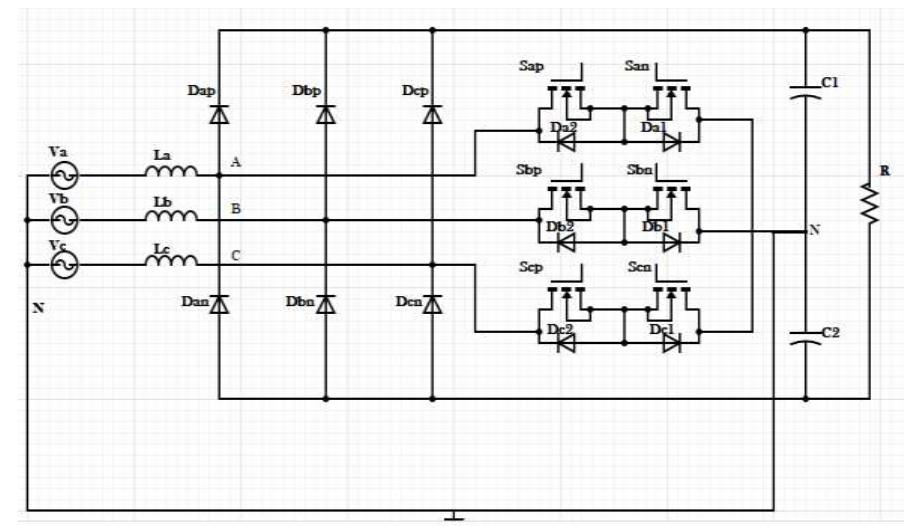
\includegraphics[width=\linewidth]{images/figure-3-phase-wire-vienna-rectifier.jpeg}
    \caption{Braço do Vienna de 4 fios.}
    \label{fig:braco_vienna}
\end{figure}

A figura \ref{fig:braco_vienna} mostra o braço do retificador de Vienna de quatro fios,
a tensão aplicada à fase é a tensão de polo $v_{kM}$, e cada fase  $k \in \{a,b,c\}$ é descrita de forma independente, como apresentado na equação \ref{eq:modelo_vienna4}.

\begin{equation}
    L\frac{di_k}{dt} = v_k - R i_k - v_{kM}, \qquad
    v_{kM} =
    \begin{cases}
        (1-d_k)V_{C1},  & i_k > 0\\
        -(1-d_k)V_{C2}, & i_k < 0
    \end{cases}
    \label{eq:modelo_vienna4}
\end{equation}

Na equação, $d_k$  é a razão cíclica da chave $S_k$. Além disso, os capacitores respeitam a
equação \ref{eq:capacitores}.

\begin{equation}
    C\frac{dV_{C1}}{dt} = \sum_{i_k>0}^{}(1-d_k)i_k-i_L, \qquad
    C\frac{dV_{C2}}{dt} = \sum_{i_k<0}^{}(1-d_k)|i_k|-i_L.
    \label{eq:capacitores}
\end{equation}

Da equação \ref{eq:modelo_vienna}, tem-se que a corrente no ponto médio ($i_M$) é a soma das correntes de cada fase, ou seja, $i_M = \sum_{}^{}d_ki_k$. 
Além disso, em regime permantente, o conversor deve sintetizar uma tensão, que no formato de fasores, pode ser representada por:

\begin{equation}
    \fasor{V}_{\sub{conv}} = \fasor{V}_s - (R + j\omega_0 L)\fasor{I}, \fasor{I} = Ae^{-j\phi},
    \label{eq:fasor}
\end{equation}

Na equação \ref{eq:fasor}, $\phi>0$ representa uma corrente atrasada. Caso $\fasor{V_{conv}}$ e $\fasor{I}$ não estejam em fase,
então para cada semiciclo, existe um intervalo em que a tensão necessária tem o sinal oposto ao da corrente
e, dessa forma, a corrente irá se distorcer em decorrência da saturação de $d_k$. Desconsideranto R na equação \ref{eq:fasor}, o alinhamento
entre a corrente e a tensão do conversor exige que $V_{pk}sin(\phi) = \omega_{0}LA$, ou seja, a corrente de linha é atrasada em relação à tensão do conversor.
Tendo isso em vista, tem-se a equação \ref{eq:phi}.

\begin{equation}
    \phi= \Psi_0 = arcsin(\omega_0LA/V_{pk})
    \label{eq:phi}
\end{equation}

Logo, o ângulo sem distorção é indutivo e cresce com a corrente.


